% Preamble with document settings and package importing
\documentclass[11pt,a4paper,twoside]{book}

\usepackage[T1]{fontenc}
\usepackage{mathpazo,courier,helvet}

\usepackage{booktabs}
\usepackage{longtable}
\usepackage{natbib}
\usepackage[titletoc,page]{appendix}

\newcommand{\var}[1]{\texttt{\${#1}}}



% Title page:
\makeatletter

\renewcommand{\maketitle}{%
  \begin{titlepage}
    {\parindent 0pt%
      {\centering
        \vfill
          \textbf{\Huge{\@title}}
        \vfill
          \Large{\@author}
        \vfill
        \vfill
          
\includegraphics[width=0.50\textwidth]{seal.uni.oslo.eps}
        \vfill
        \vfill
          \huge{Master Thesis in Informatics}
        \vfill
        \vfill
          \textsc{\Large{Department of Informatics}}
        \vfill
          \textsc{\Large{Faculty of Mathematics and Natural Sciences}}
        \vfill
          \textsc{\huge{University of Oslo}}
        \vfill
          \Large{\today}
      \par}% end centering
    }% end parindent
  \end{titlepage}
}%
\makeatother


% Document metadata
\title{Social Navigation Draft}
\author{Eivind Uggedal\\
        \texttt{eivindu@ifi.uio.no}\\\\
        % SCM stats
        }

\begin{document}
  \frontmatter
    \maketitle
    \tableofcontents
    % Include when document is of sufficient size \listoffigures
    % Include when document is of sufficient size \listoftables
  \mainmatter
    \chapter{Content Analysis}

Content analysis is a technique deployed by information architects for helping
them generate a sound and well structured website architecture. It consists of
two phases: collection of a representative sample of data and an analysis of
this content \citep[pp.~241--243]{morville06}.
A graphical content mapping can be included as an optional
intermediate phase between data inventory and analysis if one finds such
representations helpful for understanding a website's structure.
In it's essence a content analysis should identify the various
relationships (or lack of correlation) between a website's content items.
% all references needed

Instead of using content analysis as a means for improving on an existing
site's content architecture we'll be tailoring this technique to best help us
discover and understand social navigation patterns in infamous websites which
are known to make good use of such navigational designs. This means that we'll
concentrate only on core content objects and the relationships amongst them
which are organically generated---relationships which are made as part of
past users' behavior which can be leveraged by other users as a social form
of navigation.

The results of the low-level content inventories can be found in
Appendix~\ref{appendix:content.inventory}
(p.~\pageref{appendix:content.inventory}).
Particularly striking % find synonym? interesting, representative, ...
samples from graphical content mappings will be sprinkled throughout the
subsequent analysis to illustrate certain findings. The content mappings in
their full glory are located in
Appendix~\ref{appendix:content.mapping}
(p.~\pageref{appendix:content.mapping}).

\section{Flickr}

Flickr is a photo sharing site which are known to be on the cutting edge when
it comes to enabling new and innovating navigational features. This subsequent
analysis of Flickr will be carried out as a registered user. One has to be
registered for interacting with the site in such a way that one leaves
persistent traces. The site has a open nature enabling anonymous access
to the majority of content.

\sidefigure{Flickr Photo Meta-data}{%
  Photo Meta-data,
  retrieved October 28, 2007, from
  \url{http://flickr.com/photos/benbengraves/187609810/}.
}{%
  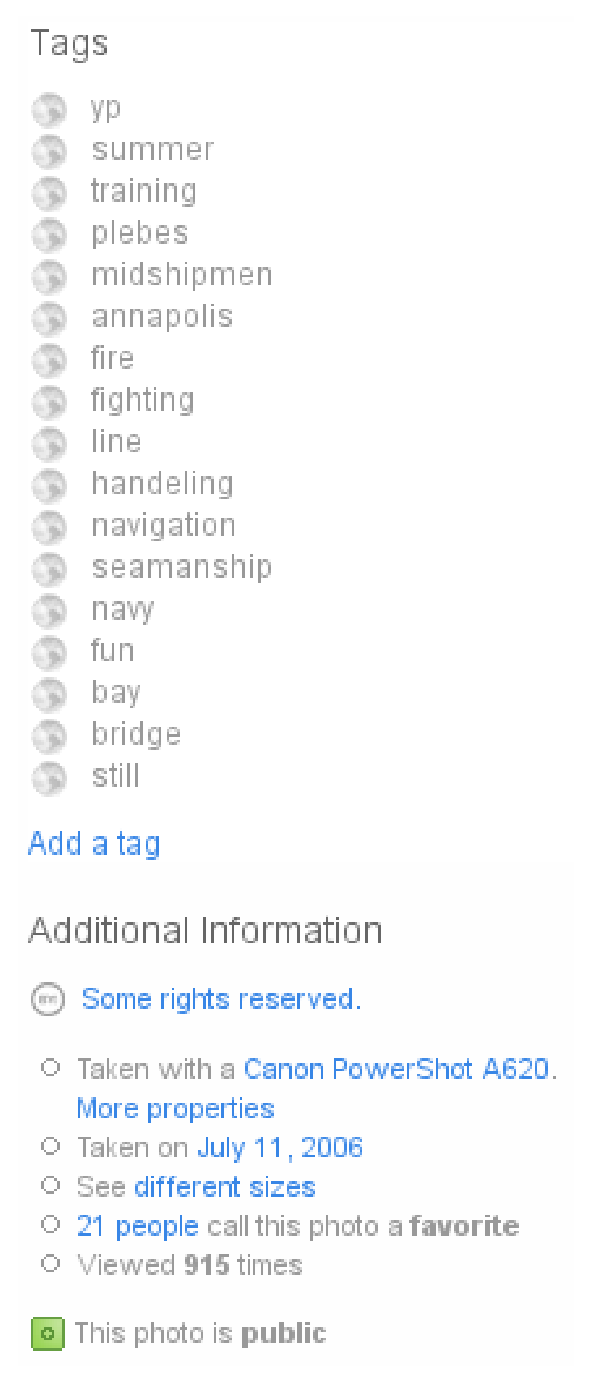
\includegraphics[width=\marginparwidth]{scrsh_flickr_photo_detail_metadata}
  \label{figure:scrsh.flickr.photo.detail.metadata}
}
            
Already on the welcome page (Figure~\ref{figure:scrsh.flickr.welcome},
p.~\pageref{figure:scrsh.flickr.welcome})
we're finding navigation links that are social of
nature. Four thumbnails functions as sample of the most recently uploaded
photos by other members of the community. One can either navigate straight to
a detailed page for each particular photo by clicking on the respective
thumbnail (Id 6, p.~\pageref{table:flickr.content.inventory.6})
or the profile of the uploader by clicking on their user
name (Id 7, p.~\pageref{table:flickr.content.inventory.7}). Such thumbnails
with minimal meta data (the uploader) are prevalent all over Flickr. Of the
120 pages we collected in our content inventory 26 of them contained
thumbnails. Most of these thumbnails%
\sidenote{Apart from the few pages that only show a
          stream of your own thumbnails--when you're browsing your
          own photos by various methods.}
are giving users incentives to navigate using social means.
Which photos these thumbnails portray is dynamic. That is to say that other
users' actions--uploading a photo, tagging a photo, taking a photo with a
specific camera, collecting photos into sets, and adding photos to a certain
group--all determine the navigational choices you as a user is
presented with.

We arrive on a photo detail page as in
Figure~\ref{figure:scrsh.flickr.photo.detail}
(p.~\pageref{figure:scrsh.flickr.photo.detail})
if we utilize one of these thumbnails for navigation. In addition to comments
on the photo we find meta-data as in 
Figure~\ref{figure:scrsh.flickr.photo.detail.metadata}
(p.~\pageref{figure:scrsh.flickr.photo.detail.metadata}). Of most importance
for Flickr, and indeed what makes Flickr a folksonomy, is tags. Every
registered user can label anyone's photos by applying such short descriptive
tags. This collaborative process lay the ground work for other user's ability
to easily browse photos by topic.
Figure~\ref{figure:scrsh.flickr.tagcloud}
(p.~\pageref{figure:scrsh.flickr.tagcloud}) exemplifies how the user generated
data trough tagging can be used as a navigational aid. A so called \emph{tag
cloud} is used to visualize the popularity (and thereby importance) of the
individual tags. The larger the tag title, the more frequent the tag has been
in use.

% Split into these sections:

\subsection{Meta-data}
% Camera specific data. Most triggered when the user decides to use a certain
% camera (or maby even when he buys a new camera at the store). But date based
% data are guided by the users desire to take a photo at a particular time.

\subsection{Folksonomy}
% most important, basis for geo i early days with geo tagging and third party
% services (citation needed). Cite interview with co-founder about it's
% importance and findability it provides. Write about clustering, it's
% principles and what it provides. Cite when it was introduced.

\subsection{Geographical data}
% Write about early geo tagging here. Write about the new places feature.
% Write and cite when proper geo data was incorporated.


\begin{figure}[b]
  \captionstyle{\raggedright}
  \centering
  \strictpagechecktrue
  \begin{adjustwidth*}{0em}{-\wholemargin}
    \begin{minipage}[t]{0.475\wholewidth}
      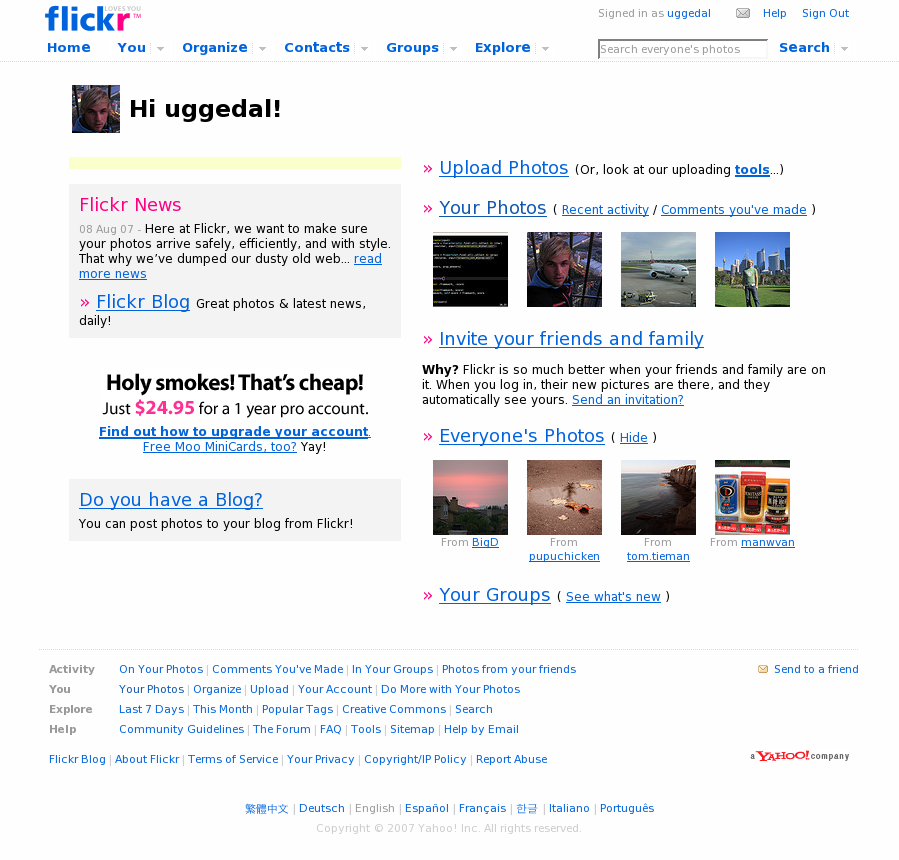
\includegraphics[width=\textwidth]{scrsh_flickr_welcome}
      \caption[Flickr Welcome Page]{%
         The Welcome Page,
         retrieved October 16, 2007, from \url{http://flickr.com}.}
      \label{figure:scrsh.flickr.welcome}
    \end{minipage}
    \hfill
    \begin{minipage}[t]{0.475\wholewidth}
      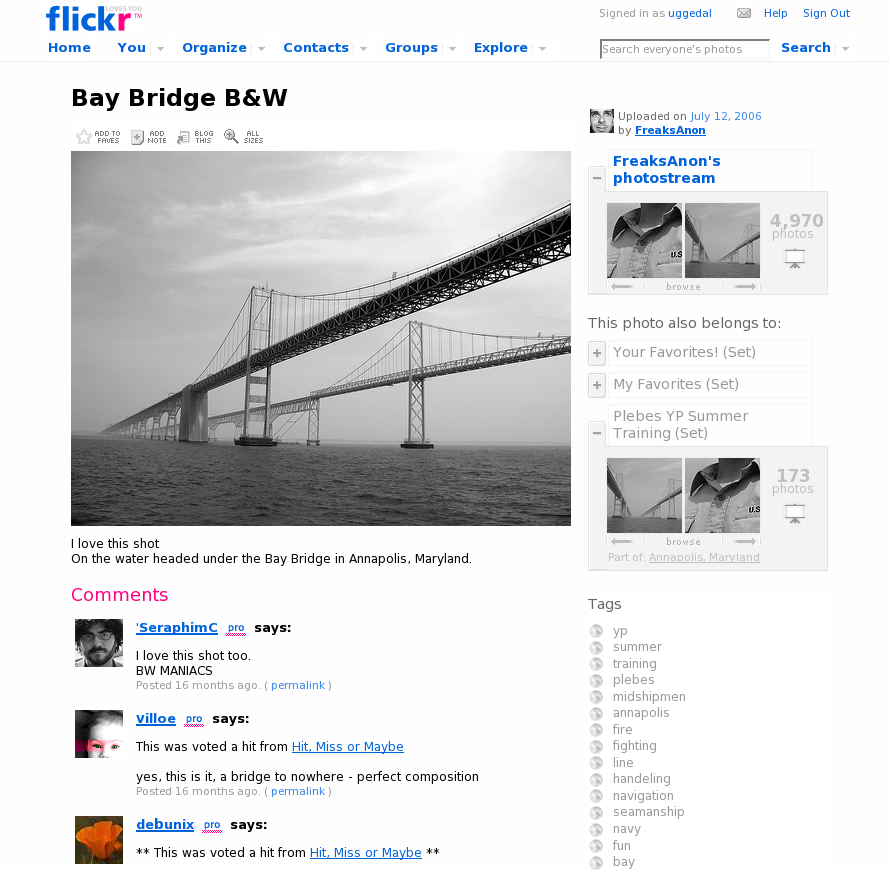
\includegraphics[width=\textwidth]{scrsh_flickr_photo_detail}
      \caption[Flickr Photo Detail Page]{%
         A Photo Detail Page,
         retrieved October 26, 2007, from
         \url{http://flickr.com/photos/benbengraves/187609810}.}
      \label{figure:scrsh.flickr.photo.detail}
    \end{minipage}
  \end{adjustwidth*}
  \normalcaption
\end{figure}

\begin{figure}
  \centering
  \strictpagechecktrue
  \begin{adjustwidth*}{0em}{-\wholemargin}
    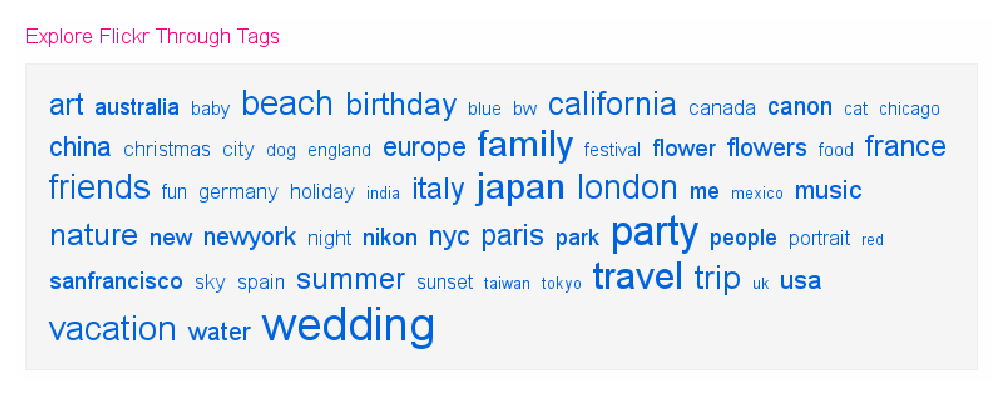
\includegraphics[width=\wholewidth]{scrsh_flickr_tagcloud}
    \caption[Flickr Tag Cloud]{%
       Tag Cloud,
       retrieved November 1, 2007, from \url{http://flickr.com/explore}.}
    \label{figure:scrsh.flickr.tagcloud}
  \end{adjustwidth*}
\end{figure}



    \chapter{Reference Test}
    Here is some textual citation of \citet{bush45}.

    Here is a paranthesized citation of \citep{dieberger97}.

    Here is some textual citation of \citet{dieberger00} and the same
    citation with all authors' names included \citet*{dieberger00}.

    Here is a textual citation of several sources
    \citet{dourish94,golder05}.

    Here is some paranthesized citation of \citet{hill92} and the same
    citation with all authors' names included \citet*{hill92}.

    Here is a paranthesized citation of several sources
    \citep{hill94,ohalloran07}.

    Here is a paranthesized citation with additional prefix text
    \citep[online from]{places07}.

    Here we just retrieve the author of a citation \citeauthor{wexelblat99}.

    \begin{appendices}
      \chapter{Content Inventory}
\label{appendix:content.inventory}

\section{Flickr}

The following content inventory detailed in
\tableref{flickr.content.inventory}
represents the state of the Flickr web site as of the 20th of September 2007.
The information we've collected could very well have changed since then as
web sites like these are known to have a rapid development cycle
where changes often are imposed on the user base at quite
a frequent rate.

As detailed in \sectionref{methodology.content.analysis.sampling}
we introduced variables for abstracting
similar page. A complete listing of such variables for Flickr and their
meaning can be found in
\tableref{flickr.variable.list}.

\begin{table}
  \begin{whole}
    \begin{tabular}{ll}

      Variable & Description \\
      \midrule

      \var{user} &
      Unique nick-name for a user \\

      \var{photo-id} &
      Unique numerical identifier for a photo \\

      \var{photo-title} &
      Textual title of a photo \\

      \var{set-id} &
      Unique numerical identifier for a set (of photos) \\

      \var{set-title} &
      Textual title of a set (of photos) \\

      \var{tag} &
      Unique name for a tag \\

      \var{group} &
      Unique textual name for a group \\

      \var{camera-make} &
      Manufacturer of digital cameras \\

      \var{camera-model} &
      Model number of a particular digital camera \\

      \var{date} &
      A given date (year, optional month, and optional day) \\

      \var{topic-id} &
      Unique numerical identifier for a discussion topic \\

      \var{topic-title} &
      Textual title of a discussion topic \\

      \var{member-count} &
      A variable number of members of a group \\

      \var{license-type} &
      One of several different \project{Creative Commons} licenses \\

    \end{tabular}
    \caption[Variable Listing for Flickr]{%
             Variables used in Flickr inventory}
    \label{table:flickr.variable.list}
  \end{whole}
\end{table}

When starting the content inventory of Flickr it became apparent that the
architects had chosen to use a \abbr{REST}ful
approach for their \abbr{URL}s.
\sidenote{
  A system that adheres to the principles of \abbr{REST}
  (Representational State Transfer)
  \citep[\p{76}]{fielding00} are sometimes called
  \abbr{REST}ful. Such principles can be applied to \abbr{URL}s
  making them represent resources
  \citep[\p{110}]{fielding00}.
}
The sites' structure was
clearly illustrated by the hierarchy of directories represented in the
\abbr{URL}. As noted in \chapterref{methodology} we took note of the
\abbr{URL}s as an aid during
our inventory phase, but decided not to display them in this thesis.


% Long multi-page table
\begin{landscape}
  \begin{footnotesize}
    \begin{longtable}{r>{\raggedright}p{7cm}ll}
      \caption{Content Inventory of Flickr}%
      \label{table:flickr.content.inventory} \\

  % First page header
  Id & Page Title & Link Name & Link Location \\
  \midrule
  \endfirsthead

  % Remaining pages header
  \caption[]{(continued)}\\
  Id & Page Title & Link Name & Link Location \\
  \midrule
  \endhead

  % Footer except for last page
  \multicolumn{4}{l}{{\emph{Continued on the next page}\ldots}} \\
  \endfoot

  % Last page footer
  \endlastfoot

  % Data

0 &
Welcome Page &
&
\\
% /

1 &
Photos from \var{user} &
You &
Global navigation \\
% /photos/\var{user}

  1.1 &
  Photo detail: \var{photo-title} &
  Photo thumbnail &
  Content area \\
  % /photos/\var{user}/\var{photo-id}

    1.1.1 &
    Photos from \var{user} &
    \var{user} &
    Content (comments list) \\
    % /photos/\var{user}

    1.1.2 &
    Photoset: \var{set-title} &
    \var{set-title} (Set) &
    Right sidebar \\
    % /photos/\var{user}/sets/\var{set-id}

    1.1.3 &
    \var{group}'s pool &
    \var{group} (Pool) &
    Right sidebar \\
    % /groups/\var{group}/pool

    1.1.4 &
    \var{user}'s photos tagged with \var{tag} &
    \var{tag} &
    Right sidebar (tag list) \\
    % /photos/\var{user}/tags/\var{tag}

      1.1.4.1 &
      All photos tagged with \var{tag} &
      public photos tagged with \var{tag} &
      Left sidebar \\
      % /photos/tags/\var{tag}

    1.1.5 &
    \var{user}'s geotagged photos on a Map &
    View \var{user} map &
    Right sidebar (details list) \\
    % /photos/\var{user}/\var{photo-id}/map/?view=users

    \label{table:flickr.content.inventory.1.1.6}
    1.1.6 &
    Everyone's geotagged photos on a Map &
    see more photos here &
    Right sidebar (details list) \\
    % /photos/\var{user}/\var{photo-id}/map/?view=everyone

    1.1.7 &
    Camera finder: \var{camera-model} &
    \var{camera-model} &
    Right sidebar (detail list) \\
    % /cameras/\var{camera-make}/\var{camera-model}

    1.1.8 &
    Archive of \var{user}'s photos taken on \var{date} &
    \var{camera-model} &
    Right sidebar (detail list) \\
    % /photos/\var{user}/archives/date-taken/\var{date}

  1.2 &
  Photoset: \var{set-title} &
  \var{set-title} &
  Left sidebar \\
  % /photos/\var{user}/sets/\var{set-id}

  1.3 &
  \var{user}'s photosets &
  Sets &
  Local navigation \\
  % /photos/\var{user}/sets

    1.3.1 &
    Photoset: \var{set-title} &
    \var{set-title} &
    Content area \\
    % /photos/\var{user}/sets/\var{set-id}

      1.1.1.1 &
      Photo detail in set: \var{photo-title} &
      Photo thumbnail &
      Content area \\
      % /photos/\var{user}/\var{photo-id}/in/set-\var{set-id}

  1.4 &
  \var{user}'s tags &
  Tags &
  Local navigation \\
  % /photos/\var{user}/tags

    1.4.1 &
    \var{user}'s photos tagged with \var{tag} &
    \var{tag} &
    Content (tag cloud) \\
    % /photos/\var{user}/tags/\var{tag}

      1.4.1.1 &
      All photos tagged with \var{tag} &
      public photos tagged with \var{tag} &
      Left sidebar \\
      % /photos/tags/\var{tag}

      1.4.1.2 &
      Photo detail: \var{photo-title} &
      Photo thumbnail &
      Content area \\
      % /photos/\var{user}/\var{photo-id}

  1.5 &
  \var{user}'s geotagged photos on a Map &
  Map &
  Local navigation \\
  % /photos/\var{user}/map

    1.5.1 &
    Photo detail on map: \var{photo-title} &
    Photo count icon &
    Map \\
    % /photos/\var{user}/map

      1.5.1.1 &
      \var{user}'s photos tagged with \var{tag} &
      \var{tag} &
      In-line dialog \\
      % /photos/\var{user}/tags/\var{tag}

      1.5.1.2 &
      Photo detail: \var{photo-title} &
      View photo page &
      In-line dialog \\
      % /photos/\var{user}/\var{photo-id}

  1.6 &
  Archive of \var{user}'s photos on Flickr &
  Archives &
  Local navigation \\
  % /photos/\var{user}/archives

    1.6.1 &
    Archive of \var{user}'s photos taken on \var{date} &
    \var{date} &
    Content area (Taken on) \\
    % /photos/\var{user}/archives/date-taken/\var{date}

      1.6.1.1 &
      Photo detail: \var{photo-title} &
      Photo thumbnail &
      Content area \\
      % /photos/\var{user}/\var{photo-id}

    1.6.2 &
    Archive of \var{user}'s photos posted on \var{date} &
    \var{date} &
    Content area (Posted on) \\
    % /photos/\var{user}/archives/date-posted/\var{date}

      1.6.2.1 &
      Photo detail: \var{photo-title} &
      Photo thumbnail &
      Content area \\
      % /photos/\var{user}/\var{photo-id}

  1.7 &
  \var{user}'s favorite photos on Flickr &
  Favorites &
  Local navigation \\
  % /photos/\var{user}/favorites

    1.7.1 &
    Photo detail: \var{photo-title} &
    Photo thumbnail &
    Content area \\
    % /photos/\var{user}/\var{photo-id}

  1.8 &
  \var{user}'s most popular photos, interestingness &
  Popular &
  Local navigation \\
  % /photos/\var{user}/popular-interesting

    1.8.1 &
    Photo detail: \var{photo-title} &
    Photo thumbnail or photo title &
    Content area \\
    % /photos/\var{user}/\var{photo-id}

    1.8.2 &
    \var{user}'s most popular photos, views &
    Views &
    Sub local navigation \\
    % /photos/\var{user}/popular-views

      1.8.2.1 &
      Photo detail: \var{photo-title} &
      Photo thumbnail or photo title &
      Content area \\
      % /photos/\var{user}/\var{photo-id}

    1.8.3 &
    \var{user}'s most popular photos, favorites &
    Favorites &
    Sub local navigation \\
    % /photos/\var{user}/popular-faves

      1.8.3.1 &
      Photo detail: \var{photo-title} &
      Photo thumbnail or photo title &
      Content area \\
      % /photos/\var{user}/\var{photo-id}

    1.8.4 &
    \var{user}'s most popular photos, comments &
    Comments &
    Sub local navigation \\
    % /photos/\var{user}/popular-comments

      1.8.4.1 &
      Photo detail: \var{photo-title} &
      Photo thumbnail or photo title &
      Content area \\
      % /photos/\var{user}/\var{photo-id}

  1.9 &
  Profile: \var{user} &
  Profile &
  Local navigation \\
  % /people/\var{user}

    1.9.1 &
    Photos from \var{user} &
    \var{user} &
    Content (Groups) \\
    % /photos/\var{user}

    1.9.2 &
    Group: \var{group} &
    \var{group} &
    Content (Groups) \\
    % /groups/\var{group}

2 &
Organize your photos &
Organize &
Global navigation \\
% /photos/organize

3 &
Photos from your contacts &
Contacts &
Global navigation \\
% /photos/friends

  3.1 &
  Photo detail: \var{photo-title} &
  Photo thumbnail &
  Content area \\
  % /photos/\var{user}/\var{photo-id}

  3.2 &
  Photos from \var{user} &
  \var{user} &
  Content area \\
  % /photos/\var{user}

4 &
Groups &
Groups &
Global navigation \\
% /groups

  4.1 &
  Group: \var{group} &
  \var{group} &
  Content \\
  % /groups/\var{group}

    4.1.1 &
    Discussion: \var{group} &
    Discussion &
    Local navigation \\
    % /groups/\var{group}/discuss

      4.1.1.1 &
      Topic: \var{topic-title} in \var{group} &
      \var{topic-title} &
      Content (topic list) \\
      % /groups/\var{group}/discuss/\var{topic-id}

      4.1.1.2 &
      Photos from \var{user} &
      \var{user} &
      Content (topic list) \\
      % /photos/\var{user}

    4.1.2 &
    \var{group}'s pool &
    Pool &
    Local navigation \\
    % /groups/\var{group}/discuss

      4.1.2.1 &
      Photo detail: \var{photo-title} &
      Photo thumbnail &
      Content area \\
      % /photos/\var{user}/\var{photo-id}/in/pool-\var{group}

      4.1.2.2 &
      Photos from \var{user} &
      \var{user} &
      Content area \\
      % /photos/\var{user}

    4.1.3 &
    Geotagged photos from \var{group}  &
    Pool &
    Local navigation \\
    % /groups/\var{group}/pool/map?mode=group

      4.1.3.1 &
      Photo detail on map: \var{photo-title} &
      Photo count icon &
      Map \\
      % /groups/\var{group}/pool/map?mode=group

        4.1.3.1.1 &
        \var{user}'s photos tagged with \var{tag} &
        \var{tag} &
        In-line dialog \\
        % /photos/\var{user}/tags/\var{tag}

        4.1.3.1.2 &
        Photo detail: \var{photo-title} &
        View photo page &
        In-line dialog \\
        % /photos/\var{user}/\var{photo-id}

    4.1.3 &
    Members of \var{group} &
    \var{member-count} Members &
    Local navigation \\
    % /groups\_members.gne?id=\var{group}-id

      4.1.3.1 &
      Photos from \var{user} &
      \var{user} &
      Content area \\
      % /photos/\var{user}

5 &
Explore &
Explore &
Global navigation \\
% /explore

  5.1 &
  Photo detail: \var{photo-title} &
  Photo thumbnail or \var{photo-title} &
  Content (highlighted photo) \\
  % /photos/\var{user}/\var{photo-id}

  5.2 &
  Photos from \var{user} &
  \var{user} &
  Content (highlighted photo) \\
  % /photos/\var{user}

  \label{table:flickr.content.inventory.5.3}
  5.3 &
  Interesting photos from the last 7 days &
  last 7 days &
  Content area \\
  % /explore/interesting/7days

    5.3.1 &
    Photo detail: \var{photo-title} &
    Photo thumbnail or \var{photo-title} &
    Content area \\
    % /photos/\var{user}/\var{photo-id}

    5.3.2 &
    Photos from \var{user} &
    \var{user} &
    Content area \\
    % /photos/\var{user}

  \label{table:flickr.content.inventory.5.4}
  5.4 &
  Interesting photos from \var{date} &
  \var{date} &
  Content area \\
  % /explore/interesting/\var{date}

    5.4.1 &
    Photo detail: \var{photo-title} &
    Photo thumbnail or \var{photo-title} &
    Content area \\
    % /photos/\var{user}/\var{photo-id}

    5.4.2 &
    Photos from \var{user} &
    \var{user} &
    Content area \\
    % /photos/\var{user}

  5.5 &
  Everyone's geotagged photos on a Map &
  a map of the world &
  Content area \\
  % /map

    5.5.1 &
    Photo detail on map: \var{photo-title} &
    Photo count icon &
    Map \\
    % /map

      5.5.1.1 &
      \var{user}'s photos tagged with \var{tag} &
      \var{tag} &
      In-line dialog \\
      % /photos/\var{user}/tags/\var{tag}

      5.5.1.2 &
      Photo detail: \var{photo-title} &
      View photo page &
      In-line dialog \\
      % /photos/\var{user}/\var{photo-id}

  5.6 &
  Popular Tags &
  popular tags &
  Content area \\
  % /photos/tags

    5.6.1 &
    Photos tagged with \var{tag} &
    \var{tag} &
    Content (tag cloud) \\
    % /photos/tags/\var{tag}

      5.6.1.1 &
      Photos tagged with \var{tag} &
      Most interesting &
      Left column \\
      % /photos/tags/\var{tag}/interesting

        5.6.1.1.1 &
        Photo detail: \var{photo-title} &
        Photo thumbnail &
        Content area \\
        % /photos/\var{user}/\var{photo-id}

        5.6.1.1.2 &
        Photos from \var{user} &
        \var{user} &
        Content area \\
        % /photos/\var{user}

      5.6.1.2 &
      Clusters for \var{tag} &
      \var{tag} clusters &
      Left column \\
      % /photos/tags/\var{tag}/clusters

        5.6.1.2.1 &
        Photo detail: \var{photo-title} &
        Photo thumbnail &
        Content area \\
        % /photos/\var{user}/\var{photo-id}

        5.6.1.2.2 &
        Photos from \var{user} &
        \var{user} &
        Content area \\
        % /photos/\var{user}

        5.6.1.2.3 &
        Clusters for \var{tag} &
        \var{tag} &
        Content (cluster list) \\
        % /photos/tags/\var{tag}/clusters

        5.6.1.2.4 &
        Photos in cluster: \var{tag} \var{tag} \var{tag} &
        See more of this cluster\ldots &
        Content area \\
        % /photos/tags/\var{tag}/clusters/\var{tag}-\var{tag}-\var{tag}

          5.6.1.2.4.1 &
          Photo detail: \var{photo-title} &
          Photo thumbnail &
          Content area \\
          % /photos/\var{user}/\var{photo-id}

          5.6.1.2.4.2 &
          Photos from \var{user} &
          \var{user} &
          Content area \\
          % /photos/\var{user}

      5.6.1.3 &
      Photo detail: \var{photo-title} &
      Photo thumbnail &
      Content area \\
      % /photos/\var{user}/\var{photo-id}

      5.6.1.4 &
      Photos from \var{user} &
      \var{user} &
      Content area \\
      % /photos/\var{user}

  5.7 &
  Camera Finder &
  Camera finder &
  Content area \\
  % /cameras

    5.7.1 &
    Camera finder: \var{camera-make} &
    \var{camera-make} &
    Content area \\
    % /cameras/\var{camera-make}

      5.7.1.1 &
      Camera finder: \var{camera-make}: \var{camera-model} &
      \var{camera-model} &
      Content area \\
      % /cameras/\var{camera-make}/\var{camera-model}

        5.7.1.1.1 &
        Photo detail: \var{photo-title} &
        Photo thumbnail &
        Content area \\
        % /photos/\var{user}/\var{photo-id}

        5.6.1.1.2 &
        Photos from \var{user} &
        \var{user} &
        Content area \\
        % /photos/\var{user}

  5.8 &
  Photos from everyone &
  most recent uploads &
  Content area \\
  % /photos

      5.8.1 &
      Photo detail: \var{photo-title} &
      Photo thumbnail &
      Content area \\
      % /photos/\var{user}/\var{photo-id}

      5.8.2 &
      Photos from \var{user} &
      \var{user} &
      Content area \\
      % /photos/\var{user}

      5.8.3 &
      Popular Tags &
      Popular tags &
      Right sidebar \\
      % /photos/tags

      5.8.4 &
      Creative Commons &
      Creative Commons &
      Right sidebar \\
      % /creativecommons

        5.8.4.1 &
        Photo detail: \var{photo-title} &
        Photo thumbnail &
        Content area \\
        % /photos/\var{user}/\var{photo-id}

        5.8.4.2 &
        Photos from \var{user} &
        \var{user} &
        Content area \\
        % /photos/\var{user}

        5.8.4.3 &
        Photos with Creative Commons \var{license-type} &
        See more &
        Content (\var{license-type} \\
        % /photos/\var{user}

          5.8.4.3.1 &
          Photo detail: \var{photo-title} &
          Photo thumbnail &
          Content area \\
          % /photos/\var{user}/\var{photo-id}

          5.8.4.3.2 &
          Photos from \var{user} &
          \var{user} &
          Content area \\
          % /photos/\var{user}

  5.9 &
  Photos tagged with \var{tag} &
  \var{tag} &
  Content (tag cloud) \\
  % /photos/tags/\var{tag}

  5.10 &
  Interesting photos from \var{date} &
  \var{date} &
  Content (A year ago) \\
  % /explore/interesting/\var{date}

    5.10.1 &
    Photo detail: \var{photo-title} &
    Photo thumbnail &
    Content area \\
    % /photos/\var{user}/\var{photo-id}

    5.10.2 &
    Photos from \var{user} &
    \var{user} and see more photos &
    Content area \\
    % /photos/\var{user}

    5.10.3 &
    Profile: \var{user} &
    profile &
    Content area \\
    % /people/\var{user}

    5.10.4 &
    Clusters for \var{tag} &
    \var{tag} &
    Content area \\
    % /photos/tags/\var{tag}/clusters

  5.11 &
  Photo detail: \var{photo-title} &
  Photo thumbnail or \var{photo-title} &
  Content (A year ago) \\
  % /photos/\var{user}/\var{photo-id}

  5.12 &
  Photos from \var{user} &
  \var{user} &
  Content (A year ago) \\
  % /photos/\var{user}

  5.13 &
  Profile: \var{user} &
  profile &
  Content (A year ago) \\
  % /people/\var{user}

  5.14 &
  Photoset: \var{set-title} &
  \var{set-title} &
  Content (Sets) \\
  % /photos/\var{user}/sets/\var{set-id}

    5.14.1 &
    Photo detail in set: \var{photo-title} &
    Photo thumbnail &
    Content area \\
    % /photos/\var{user}/\var{photo-id}/in/set-\var{set-id}

  5.15 &
  Photos from \var{user} &
  \var{user} &
  Content (Sets) \\
  % /photos/\var{user}

  5.16 &
  Groups &
  loads of groups &
  Content (Groups) \\
  % /groups

  5.17 &
  Group: \var{group} &
  \var{group} &
  Content (Groups) \\
  % /groups/\var{group}

  5.18 &
  \var{group}'s pool &
  Pool &
  Local navigation \\
  % /groups/\var{group}/pool

  5.19 &
  Members of \var{group}  &
  \var{member-count} Members &
  Local navigation \\
  % /groups\_members.gne?id=\var{group}-id

6 &
\label{table:flickr.content.inventory.6}
Photo detail: \var{photo-title} &
Photo thumbnail &
Content area \\
% /photos/\var{user}/\var{photo-id}

7 &
\label{table:flickr.content.inventory.7}
Photos from \var{user} &
\var{user} &
Content area \\
% /photos/\var{user}


    \end{longtable}
  \end{footnotesize}
\end{landscape}


\section{Facebook}

The inventory of the Facebook web site represents the state it was in
the 14th of May 2008. We're also using variables for our Facebook inventory
and their representations can be found in
\tableref{facebook.variable.list}.

\begin{table}
  \begin{whole}
     \begin{tabular}{lp{20pc}l}

      Variable & Description \\
      \midrule

      \var{person} &
      Full name of a person \\

      \var{network} &
      The name of a network \\

      \var{group} &
      The name of a group \\

      \var{member-count} &
      A variable number of members of a group or network \\

      \var{photo-count} &
      A variable number of photos \\

      \var{video} &
      Title of a video \\

      \var{video-count} &
      A variable number of videos \\

      \var{posted-count} &
      A variable number of posted items \\

      \var{comment-count} &
      A variable number of comments on a posted item \\

      \var{discussion-topic} &
      Topic of a discussion topic in a discussion board \\

      \var{discussion-count} &
      A variable number of discussions on a discussion board \\

      \var{event} &
      The name of an event \\

      \var{guest-count} &
      A variable number of events \\

      \var{guest-count} &
      A variable number of guest for an event \\

      \var{wall-post-count} &
      A variable number of posts on a wall \\

      \var{classified} &
      The name of a classified in the marketplace \\

      \var{gender} &
      The sex of a person: male, female, or unspecified \\

      \var{relationship} &
      Status of a persons relationship:
      Single, in a relationship, engaged, married,
      it's complicated, or in an open relationship. \\

      \var{gender-interest} &
      What gender a person is interested in: men or women. \\

      \var{looking-for} &
      What a person is looking for from other people:
      friendship, dating, a relationship, or networking.\\

      \var{birth-date} &
      The date of a person's birth \\

      \var{birth-year} &
      The year of a person's birth \\

      \var{home-town} &
      The town a person calls home \\

      \var{home-country} &
      The country a person calls home \\

      \var{political-view} &
      A person's political view: very liberal, liberal
      moderate, conservative, very conservative,
      apathetic, libertarian, or other.\\

      \var{religious-view} &
      A person's religious view. \\

      \var{album} &
      Title of a photo album. \\

      \var{album-count} &
      A variable number of photo albums. \\

      \var{page} &
      Title of a fan page. \\

      \var{fan-count} &
      A variable number of fans of a fan page. \\

    \end{tabular}
    \caption[Variable Listing for Facebook]{%
             Variables used in Facebook inventory}
    \label{table:facebook.variable.list}
  \end{whole}
\end{table}

Note that we've described the users of Facebook as people. At Flickr one can
have an online, almost anonymous, nickname. On Facebook on the other hand one
have to provide a real name%
\sidenote{
  \postquote{facebook08a}{%
    Facebook disallows certain names and words in names that tend to be
    associated with fake accounts (e.g. Paris Hilton)}
}
and the account have to represent an existing individual%
\sidenote{
  \postquote{facebook08a}{%
    using the name of a group or organization is not permitted, as
    Facebook accounts are for individual use only}
}.


% Long multi-page table
\begin{landscape}
  \begin{footnotesize}
    \begin{longtable}{r>{\raggedright}p{7cm}ll}
      \caption{Content Inventory of Flickr}%
      \label{table:facebook.content.inventory} \\

  % First page header
  Id & Page Title & Link Name & Link Location \\
  \midrule
  \endfirsthead

  % Remaining pages header
  \caption[]{(continued)}\\
  Id & Page Title & Link Name & Link Location \\
  \midrule
  \endhead

  % Footer except for last page
  \multicolumn{4}{l}{{\emph{Continued on the next page}\ldots}} \\
  \endfoot

  % Last page footer
  \endlastfoot

  % Data

\label{table:facebook.content.inventory.0}
0 &
Home &
Login form &
Login page \\
% /home.php?

\label{table:facebook.content.inventory.1}
1 &
\var{person} &
Profile &
Global navigation \\
% /profile.php?id=\var{person-id}

  1.1 &
  My networks &
  \var{network} &
  Person info box \\
  % /networks/\var{network-id}\var{network}

    1.1.1 &
    Browse My Networks &
    \var{member-count} &
    Network info box \\
    % /b.php?n=\var{network-id}&new

      1.1.1.1 &
      \var{person} &
      Profile picture  &
      Member list \\
      % /profile.php?id=\var{person-id}

      1.1.1.2 &
      \var{person} &
      \var{person} &
      Member list \\
      % /profile.php?id=\var{person-id}

      1.1.1.3 &
      \var{network} &
      \var{network} &
      Member list \\
      % /networks/\var{network-id}\var{network}

      1.1.1.4 &
      \var{network} &
      Send message &
      Member list \\
      % /inbox/?compose&id=\var{user-id}

      1.1.1.5 &
      \var{person}'s Friends &
      View Friends &
      Member list \\
      % /friends/?id=\var{person-id}

        1.1.1.5.1 &
        \var{person} &
        Profile picture  &
        Member list \\
        % /profile.php?id=\var{person-id}

        1.1.1.5.2 &
        \var{person} &
        \var{person} &
        Member list \\
        % /profile.php?id=\var{person-id}

    1.1.2 &
    Networks on Facebook &
    Browse Networks &
    Network info box \\
    % /networks/networks.php

      1.1.2.1 &
      \var{network} &
      \var{network} &
      Network List \\
      % /networks/\var{network-id}\var{network}

    1.1.3 &
    Popular Today (Posted Items) &
    See What's Popular &
    Network info box \\
    % /networks/activity.php?nk=\var{network-id}&rt=0&ot=2

      1.1.3.1 &
      Popular Today (Groups) &
      Groups &
      Global content area navigation \\
      % /networks/activity.php?nk=\var{network-id}&rt=0&ot=0

        1.1.3.1.1 &
        \var{group} &
        Group picture  &
        Group list \\
        % /group.php?gid=\var{group-id}

          1.1.3.1.1.1 &
          Photos from \var{group} &
          \var{photo-count} &
          Photo box \\
          % /photo_search.php?oid=\var{group-id}&view=all

            1.1.3.1.1.1.1 &
            Photos from \var{group} (View single) &
            Photo thumbnail &
            Photos list \\
            % /photo.php?pid=\var{photo-id}&op=1&o=all&view=all&subj=\var{group-id}&aid=-1&oid=\var{group-id}&id=26609908#pid=32079027&id=26609908

              1.1.3.1.1.1.1.1 &
              Photos from \var{group} (View single) &
              Previous &
              Photo navigation \\
              % /photo.php?pid=\var{photo-id}&op=1&o=all&view=all&subj=\var{group-id}&aid=-1&oid=\var{group-id}&id=26609908#pid=32079027&id=26609908

              1.1.3.1.1.1.1.2 &
              Photos from \var{group} (View single) &
              Next &
              Photo navigation \\
              % /photo.php?pid=\var{photo-id}&op=1&o=all&view=all&subj=\var{group-id}&aid=-1&oid=\var{group-id}&id=26609908#pid=32079027&id=26609908

              1.1.3.1.1.1.1.3 &
              \var{person} &
              \var{person} &
              Tagged people in photo \\
              % /profile.php?id=\var{person-id}

              1.1.3.1.1.1.1.4 &
              \var{person} &
              Added by \var{person} &
              Photo meta-data \\
              % /profile.php?id=\var{person-id}

              1.1.3.1.1.1.1.5 &
              \var{person} &
              Profile picture  &
              Comment \\
              % /profile.php?id=\var{person-id}

              1.1.3.1.1.1.1.6 &
              \var{person} &
              \var{person} &
              Comment \\
              % /profile.php?id=\var{person-id}

          1.1.3.1.1.2 &
          Photos from \var{group} &
          See All &
          Photos box \\
          % /photo_search.php?oid=\var{group-id}&view=all

          1.1.3.1.1.3 &
          Videos from \var{group} &
          \var{video-count} &
          Videos box \\
          % /video/?oid=\var{group-id}

            1.1.3.1.1.3.1 &
            Videos from \var{group} \var{video} &
            Video thumbnail &
            Video list \\
            % /video/video.php?v=\var{video-id}&oid=\var{group-id}

              1.1.3.1.1.3.1.1 &
              Videos from \var{group} \var{video} &
              Previous &
              Video navigation \\
              % /video/video.php?v=\var{video-id}&oid=\var{group-id}

              1.1.3.1.1.3.1.2 &
              Videos from \var{group} \var{video} &
              Next &
              Video navigation \\
              % /video/video.php?v=\var{video-id}&oid=\var{group-id}

              1.1.3.1.1.3.1.3 &
              \var{person} &
              \var{person} &
              Tagged people in video \\
              % /profile.php?id=\var{person-id}

              1.1.3.1.1.3.1.4 &
              \var{person} &
              Added by \var{person} &
              Video meta-data \\
              % /profile.php?id=\var{person-id}

              1.1.3.1.1.3.1.5 &
              \var{person} &
              Profile picture  &
              Comment \\
              % /profile.php?id=\var{person-id}

              1.1.3.1.1.3.1.6 &
              \var{person} &
              \var{person} &
              Comment \\
              % /profile.php?id=\var{person-id}

            1.1.3.1.1.3.2 &
            Videos from \var{group} \var{video} &
            \var{video} &
            Video list \\
            % /video/video.php?v=\var{video-id}&oid=\var{group-id}

            1.1.3.1.1.3.2 &
            \var{person} &
            by \var{person} &
            Video list \\
            % /profile.php?id=\var{person-id}


          1.1.3.1.1.4 &
          Videos from \var{group} &
          See All &
          Video box \\
          % /video/?oid=\var{group-id}

          1.1.3.1.1.5 &
          Posted Items on \var{group} &
          \var{posted-count} &
          Posted items box \\
          % /posted.php?id=\var{group-id}

            1.1.3.1.1.5.1 &
            Posted Items on \var{group} &
            \var{comment-count} comments &
            Posted item \\
            % /posted.php?id=\var{group-id}#\var{posted-id}

              1.1.3.1.1.5.1.1 &
              \var{person} &
              Profile picture  &
              Comment \\
              % /profile.php?id=\var{person-id}

              1.1.3.1.1.5.1.2 &
              \var{person} &
              \var{person} &
              Comment \\
              % /profile.php?id=\var{person-id}


          1.1.3.1.1.6 &
          Posted Items on \var{group} &
          See All &
          Posted items list \\
          % /posted.php?id=\var{group-id}

          1.1.3.1.1.7 &
          \var{group} Discussions &
          \var{discussion-count} discussion topics &
          Discussions list \\
          % /board.php?id=\var{group-id}

            1.1.3.1.1.7.1 &
            \var{discussion-topic} &
            \var{discussion-topic} &
            Discussions list \\
            % /topic.php?id=\var{group-id}&topic=\var{topic-id}

              1.1.3.1.1.7.1.1 &
              \var{person} &
              Profile picture  &
              Comment \\
              % /profile.php?id=\var{person-id}

              1.1.3.1.1.7.1.2 &
              \var{person} &
              \var{person} &
              Comment \\
              % /profile.php?id=\var{person-id}

          1.1.3.1.1.8 &
          Group Members &
          \var{member-count} &
          Member box \\
          % /s.php?k=\var{unknown-id}&id=\var{network-id}&gr=2

            1.1.3.1.1.8.1 &
            \var{person} &
            Profile picture  &
            Member list \\
            % /profile.php?id=\var{person-id}

            1.1.3.1.1.8.2 &
            \var{person} &
            \var{person} &
            Member list \\
            % /profile.php?id=\var{person-id}

          \label{table:facebook.content.inventory.1.1.3.1.1.9}
          1.1.3.1.1.9 &
          \var{group} Wall &
          \var{wall-post-count} &
          Wall posts list \\
          % /wall.php?id=\var{group-id}

            1.1.3.1.1.9.1 &
            \var{person} &
            Profile picture  &
            Wall post \\
            % /profile.php?id=\var{person-id}

            1.1.3.1.1.9.2 &
            \var{person} &
            \var{person} &
            Wall post \\
            % /profile.php?id=\var{person-id}

          1.1.3.1.1.10 &
          \var{person} &
          \var{person} &
          Officer list (right sidebar) \\
          % /profile.php?id=\var{person-id}

          1.1.3.1.1.11 &
          \var{person} &
          \var{person} &
          Admin list (right sidebar) \\
          % /profile.php?id=\var{person-id}

        1.1.3.1.2 &
        \var{group} &
        \var{group} &
        Group list \\
        % /group.php?gid=\var{group-id}

      1.1.3.2 &
      Popular Today (Events) &
      Events &
      Global content area navigation \\
      % /networks/activity.php?nk=\var{network-id}&rt=0&ot=1

        1.1.3.2.1 &
        \var{event} &
        Event picture  &
        Event list \\
        % /event.php?eid=\var{event-id}

          1.1.3.2.1.1 &
          Photos from \var{event} &
          \var{photo-count} &
          Photo box \\
          % /photo_search.php?oid=\var{event-id}&view=all

            1.1.3.2.1.1.1 &
            Photos from \var{event} (View single) &
            Photo thumbnail &
            Photos list \\
            % /photo.php?pid=\var{photo-id}&op=1&o=all&view=all&subj=\var{event-id}&aid=-1&oid=\var{event-id}&id=26609908#pid=32079027&id=26609908

              % same as for groups

          1.1.3.2.1.2 &
          Photos from \var{event} &
          See All &
          Photos box \\
          % /photo_search.php?oid=\var{event-id}&view=all

          1.1.3.2.1.3 &
          Videos from \var{event} &
          \var{video-count} &
          Videos box \\
          % /video/?oid=\var{event-id}

            1.1.3.2.1.3.1 &
            Videos from \var{event} \var{video} &
            Video thumbnail &
            Video list \\
            % /video/video.php?v=\var{video-id}&oid=\var{event-id}

              % same as for groups

            1.1.3.2.1.3.2 &
            Videos from \var{event} \var{video} &
            \var{video} &
            Video list \\
            % /video/video.php?v=\var{video-id}&oid=\var{event-id}

              % same as for groups

            1.1.3.2.1.3.2 &
            \var{person} &
            by \var{person} &
            Video list \\
            % /profile.php?id=\var{person-id}


          1.1.3.2.1.4 &
          Videos from \var{event} &
          See All &
          Video box \\
          % /video/?oid=\var{event-id}

          1.1.3.2.1.5 &
          Posted Items on \var{event} &
          \var{posted-count} &
          Posted items box \\
          % /posted.php?id=\var{event-id}

            1.1.3.2.1.5.1 &
            Posted Items on \var{event} &
            \var{comment-count} comments &
            Posted item \\
            % /posted.php?id=\var{event-id}#\var{posted-id}

              % same as for group

          1.1.3.2.1.6 &
          Posted Items on \var{event} &
          See All &
          Posted items list \\
          % /posted.php?id=\var{event-id}

          1.1.3.2.1.8 &
          Event Guests &
          \var{guest-count} &
          Guests box \\
          % /s.php?k=\var{unknown-id}&id=\var{network-id}&gr=2

            1.1.3.2.1.8.1 &
            \var{person} &
            Profile picture  &
            Member list \\
            % /profile.php?id=\var{person-id}

            1.1.3.2.1.8.2 &
            \var{person} &
            \var{person} &
            Member list \\
            % /profile.php?id=\var{person-id}

          \label{table:facebook.content.inventory.1.1.3.2.1.9}
          1.1.3.2.1.9 &
          \var{event} Wall &
          \var{wall-post-count} &
          Wall posts list \\
          % /wall.php?id=\var{event-id}

            1.1.3.2.1.9.1 &
            \var{person} &
            Profile picture  &
            Wall post \\
            % /profile.php?id=\var{person-id}

            1.1.3.2.1.9.2 &
            \var{person} &
            \var{person} &
            Wall post \\
            % /profile.php?id=\var{person-id}

          1.1.3.2.1.10 &
          \var{person} &
          \var{person} &
          Other invited list (right sidebar) \\
          % /profile.php?id=\var{person-id}

          1.1.3.2.1.10 &
          \var{person} &
          Profile picture &
          Other invited list (right sidebar) \\
          % /profile.php?id=\var{person-id}

          1.1.3.2.1.11 &
          \var{person} &
          \var{person} &
          Admin list (right sidebar) \\
          % /profile.php?id=\var{person-id}

        1.1.3.2.2 &
        \var{event} &
        \var{event} &
        Event list \\
        % /event.php?eid=\var{event-id}

      1.1.3.3 &
      Popular Today (Notes) &
      Notes &
      Global content area navigation \\
      % /networks/activity.php?nk=\var{network-id}&rt=0&ot=3

        1.1.3.3.1 &
        \var{person}'s Notes &
        \var{note} &
        Note list \\
        % /note.php?note_id=\var{note-id}&id=\var{person-id}

          1.1.3.3.1.1 &
          \var{person} &
          Profile picture &
          Note comment \\
          % /profile.php?id=\var{person-id}

          1.1.3.3.1.2 &
          \var{person} &
          \var{person} &
          Note comment \\
          % /profile.php?id=\var{person-id}

        1.1.3.3.2 &
        \var{person} &
        Profile picture &
        Note list \\
        % /profile.php?id=\var{person-id}

        1.1.3.3.3 &
        \var{person} &
        \var{person} &
        Note list \\
        % /profile.php?id=\var{person-id}

    1.1.4 &
    Discussions &
    View Discussion Board &
    Network info box \\
    % /board.php?uid=\var{some-id}

      % same as for groups

      1.1.3.1.1.8 &
      Group Members &
      \var{member-count} &
      Member box \\
      % /s.php?k=\var{unknown-id}&id=\var{network-id}&gr=2

        1.1.3.1.1.8.1 &
        \var{person} &
        Profile picture  &
        Member list \\
        % /profile.php?id=\var{person-id}

        1.1.3.1.1.8.2 &
        \var{person} &
        \var{person} &
        Member list \\
        % /profile.php?id=\var{person-id}


    1.1.4 &
    Browse My Networks &
    \var{member-count} &
    People in \var{network} box \\
    % /b.php?n=\var{network-id}&new

    1.1.5 &
    \var{person} &
    Profile picture  &
    Member list \\
    % /profile.php?id=\var{person-id}

    1.1.6 &
    \var{person} &
    \var{person} &
    People in \var{network} box \\
    % /profile.php?id=\var{person-id}

    1.1.7 &
    \var{event} &
    \var{event-count} &
    Upcoming events box \\
    % /event.php?eid=\var{event-id}

    1.1.8 &
    \var{event} &
    \var{event} &
    Upcoming events box \\
    % /event.php?eid=\var{event-id}

    1.1.8 &
    Popular Today (Posted Items) &
    See All &
    Network info box \\
    % /networks/activity.php?nk=\var{network-id}&rt=0&ot=2

    1.1.9 &
    Popular Today (Groups) &
    See All &
    Popular in \var{network} box \\
    % /networks/activity.php?nk=\var{network-id}&rt=0&ot=0

    1.1.10 &
    \var{group} &
    \var{group} &
    Popular in \var{network} box \\
    % /group.php?gid=\var{group-id}

    1.1.11 &
    Discussions &
    \var{discussion-count} discussion topics &
    Discussion box \\
    % /board.php?uid=\var{some-id}

      % same as for groups

    1.1.12 &
    \var{discussion-topic} &
    \var{discussion-topic} &
    Discussion box \\
    % /topic.php?id=\var{group-id}&topic=\var{topic-id}

      % same as for groups

    1.1.13 &
    \var{network}'s Wall &
    \var{wall-post-count} &
    Wall posts box \\
    % /wall.php?id=\var{network-id}

      % same as for groups

    1.1.14 &
    \var{person} &
    Profile picture  &
    Wall post \\
    % /profile.php?id=\var{person-id}

    1.1.15 &
    \var{person} &
    \var{person} &
    Wall post \\
    % /profile.php?id=\var{person-id}

    1.1.16 &
    Marketplace &
    See All &
    Marketplace box \\
    % /marketplace.php?f=\var{network-id}&b=\var{some-id}

      1.1.16.1 &
      Marketplace - \var{classified} &
      \var{classified} &
      Classified listing \\
      % /marketplace/listing.php?f=\var{classified-id}

        1.1.16.1.1 &
        \var{person} &
        \var{person} &
        Classified info \\
        % /profile.php?id=\var{person-id}

      1.1.16.2 &
      \var{person} &
      \var{person} &
      Classified info \\
      % /profile.php?id=\var{person-id}

    1.1.17 &
    Marketplace - \var{classified} &
    \var{classified} &
    Marketplace box \\
    % /marketplace/listing.php?f=\var{classified-id}

  1.2 &
  Browse My networks (by gender) &
  \var{gender} &
  Person info box \\
  % /b.php?k=\var{some-id}&n=\var{some-count}&sx=\var{gender-id}&o=\var{some-count}

    1.2.1 &
    \var{person} &
    Profile picture  &
    Person listing \\
    % /profile.php?id=\var{person-id}

    1.2.2 &
    \var{person} &
    \var{person} &
    Person listing \\
    % /profile.php?id=\var{person-id}

    1.2.3 &
    My networks &
    \var{network} &
    Person listing \\
    % /networks/\var{network-id}\var{network}

  1.3 &
  Browse My networks (by gender interest) &
  \var{gender-interest} &
  Person info box \\
  % /b.php?k=\var{some-id}&n=\var{some-count}&ii=\var{gender-interest-id}&o=\var{some-count}

    1.3.1 &
    \var{person} &
    Profile picture  &
    Person listing \\
    % /profile.php?id=\var{person-id}

    1.3.2 &
    \var{person} &
    \var{person} &
    Person listing \\
    % /profile.php?id=\var{person-id}

    1.3.3 &
    My networks &
    \var{network} &
    Person listing \\
    % /networks/\var{network-id}\var{network}

  1.4 &
  Browse My networks (by relationship status) &
  \var{relationship} &
  Person info box \\
  % /b.php?k=\var{some-id}&n=\var{some-count}&rl=\var{relationship-id}&o=\var{some-count}

    1.4.1 &
    \var{person} &
    Profile picture  &
    Person listing \\
    % /profile.php?id=\var{person-id}

    1.4.2 &
    \var{person} &
    \var{person} &
    Person listing \\
    % /profile.php?id=\var{person-id}

    1.4.3 &
    My networks &
    \var{network} &
    Person listing \\
    % /networks/\var{network-id}\var{network}

  1.5 &
  Browse My networks (by looking for) &
  \var{looking-for} &
  Person info box \\
  % /b.php?k=\var{some-id}&n=\var{some-count}&if=\var{looking-for-id}&o=\var{some-count}

    1.5.1 &
    \var{person} &
    Profile picture  &
    Person listing \\
    % /profile.php?id=\var{person-id}

    1.5.2 &
    \var{person} &
    \var{person} &
    Person listing \\
    % /profile.php?id=\var{person-id}

    1.5.3 &
    My networks &
    \var{network} &
    Person listing \\
    % /networks/\var{network-id}\var{network}

  1.6 &
  Profile Search Results (by birthday) &
  \var{birth-date} &
  Person info box \\
  % /s.php?adv&k=\var{some-id}&n=\var{some-count}&67=\var{birth-date}&o=\var{some-count}

    1.6.1 &
    \var{person} &
    Profile picture  &
    Person listing \\
    % /profile.php?id=\var{person-id}

    1.6.2 &
    \var{person} &
    \var{person} &
    Person listing \\
    % /profile.php?id=\var{person-id}

    1.6.3 &
    My networks &
    \var{network} &
    Person listing \\
    % /networks/\var{network-id}\var{network}

  1.7 &
  Browse My networks (by birth year) &
  \var{birth-year} &
  Person info box \\
  % /b.php?k=\var{some-id}&n=\var{some-count}&y1=\var{age-from}&y2=\var{age-to}&o=\var{some-count}

    1.7.1 &
    \var{person} &
    Profile picture  &
    Person listing \\
    % /profile.php?id=\var{person-id}

    1.7.2 &
    \var{person} &
    \var{person} &
    Person listing \\
    % /profile.php?id=\var{person-id}

    1.7.3 &
    My networks &
    \var{network} &
    Person listing \\
    % /networks/\var{network-id}\var{network}

  1.8 &
  Profile Search Results (by home town) &
  \var{home-town} &
  Person info box \\
  % /s.php?adv&k=\var{some-id}&n=\var{some-count}&c1=\var{home-town}&o=\var{some-count}

    1.8.1 &
    \var{person} &
    Profile picture  &
    Person listing \\
    % /profile.php?id=\var{person-id}

    1.8.2 &
    \var{person} &
    \var{person} &
    Person listing \\
    % /profile.php?id=\var{person-id}

    1.8.3 &
    My networks &
    \var{network} &
    Person listing \\
    % /networks/\var{network-id}\var{network}

  1.9 &
  Profile Search Results (by home country) &
  \var{home-country} &
  Person info box \\
  % /s.php?adv&k=\var{some-id}&n=\var{some-count}&k1=\var{home-country-id}&o=\var{some-count}

    1.9.1 &
    \var{person} &
    Profile picture  &
    Person listing \\
    % /profile.php?id=\var{person-id}

    1.9.2 &
    \var{person} &
    \var{person} &
    Person listing \\
    % /profile.php?id=\var{person-id}

    1.9.3 &
    My networks &
    \var{network} &
    Person listing \\
    % /networks/\var{network-id}\var{network}

  1.10 &
  Browse My networks (by political view) &
  \var{political-view} &
  Person info box \\
  % /b.php?k=\var{some-id}&n=\var{some-count}&pl=\var{political-view-id}&o=\var{some-count}

    1.10.1 &
    \var{person} &
    Profile picture  &
    Person listing \\
    % /profile.php?id=\var{person-id}

    1.10.2 &
    \var{person} &
    \var{person} &
    Person listing \\
    % /profile.php?id=\var{person-id}

    1.10.3 &
    My networks &
    \var{network} &
    Person listing \\
    % /networks/\var{network-id}\var{network}

  1.11 &
  Profile Search Results (by religious view) &
  \var{religious-view} &
  Person info box \\
  % /s.php?adv&k=\var{some-id}&n=\var{some-count}&re=\var{religious-view}&o=\var{some-count}

    1.11.1 &
    \var{person} &
    Profile picture  &
    Person listing \\
    % /profile.php?id=\var{person-id}

    1.11.2 &
    \var{person} &
    \var{person} &
    Person listing \\
    % /profile.php?id=\var{person-id}

    1.11.3 &
    My networks &
    \var{network} &
    Person listing \\
    % /networks/\var{network-id}\var{network}

  1.12 &
  Photos of \var{person} &
  View photos of \var{person} &
  Left sidebar \\
  % /photo_search.php?id=\var{person-id}

  1.13 &
  \var{person}'s Friends &
  View \var{person}'s Friends &
  Left sidebar sidebar \\
  % /friends/?id=\var{person-id}

  1.14 &
  \var{person} &
  Profile picture  &
  Friends sidebar box \\
  % /profile.php?id=\var{person-id}

  1.15 &
  \var{person} &
  \var{person} &
  Friends sidebar box \\
  % /profile.php?id=\var{person-id}

  1.16 &
  \var{person} &
  Profile picture  &
  Mutual friends sidebar box \\
  % /profile.php?id=\var{person-id}

  1.17 &
  \var{person} &
  \var{person} &
  Mutual friends sidebar box \\
  % /profile.php?id=\var{person-id}

  1.18 &
  \var{person}'s Friends &
  View \var{person}'s Friends &
  Friends in other networks sidebar box \\
  % /friends/?id=\var{person-id}&nk=\var{some-id}

  1.19 &
  \var{person}'s Photos -- \var{album} &
  Album picture &
  Photos sidebar box \\
  % /album/?aid=\var{album-id}&id=\var{person-id}

    \label{table:facebook.content.inventory.1.19.1}
    1.19.1 &
    \var{person}'s Photos -- \var{album} &
    Photo thumbnail &
    Photos list \\
    % /photo.php?pid=\var{photo-id}&id=\var{person-id}

  1.20 &
  \var{person}'s Photos -- \var{album} &
  \var{album} &
  Photos sidebar box \\
  % /album/?aid=\var{album-id}&id=\var{person-id}

  1.21 &
  \var{page} &
  Page picture &
  Pages sidebar box \\
  % /pages/\var{pages-slug}/\var{pages-id}

    1.21.1 &
    Fans of \var{page}  &
    \var{fan-count} &
    Supporters box \\
    % /s.php?k=\var{unknown-id}&id=\var{page-id}

      1.21.1.1 &
      \var{person} &
      Profile picture  &
      Fan list \\
      % /profile.php?id=\var{person-id}

      1.21.1.2 &
      \var{person} &
      \var{person} &
      Fan list \\
      % /profile.php?id=\var{person-id}

    1.21.2 &
    Fans of \var{page}  &
    See All &
    Supporters box \\
    % /s.php?k=\var{unknown-id}&id=\var{page-id}

    1.21.3 &
    \var{person} &
    Profile picture  &
    Supporters box \\
    % /profile.php?id=\var{person-id}

    1.21.4 &
    \var{person} &
    \var{person} &
    Supporters box \\
    % /profile.php?id=\var{person-id}

    1.21.5 &
    \var{page}'s photos &
    \var{album-count} &
    Photos box \\
    % /photos.php?id=\var{page-id}&ref=pb

    1.21.6 &
    \var{page}'s photos &
    See All &
    Photos box \\
    % /photos.php?id=\var{page-id}&ref=pb

      1.21.6.1 &
      \var{page}'s Photos -- \var{album} &
      Album picture &
      Album list \\
      % /album/?aid=\var{album-id}&id=\var{page-id}

      1.21.6.2 &
      \var{page}'s Photos -- \var{album} &
      \var{album} &
      Album list \\
      % /album/?aid=\var{album-id}&id=\var{page-id}

      1.21.6.3 &
      \var{page}'s Photos -- \var{album} &
      View Album &
      Album list \\
      % /album/?aid=\var{album-id}&id=\var{page-id}

    1.21.7 &
    \var{page}'s Notes &
    \var{note} &
    Notes box \\
    % /note.php?note_id=\var{note-id}&id=\var{person-id}

    1.21.8 &
    \var{page}'s Wall &
    \var{wall-post-count} &
    Wall posts box \\
    % /wall.php?id=\var{page-id}

    1.21.9 &
    \var{page}'s Wall &
    See All &
    Wall posts box \\
    % /wall.php?id=\var{page-id}

    1.21.3 &
    \var{person} &
    Profile picture  &
    Wall posts box \\
    % /profile.php?id=\var{person-id}

    1.21.4 &
    \var{person} &
    \var{person} &
    Wall posts box \\
    % /profile.php?id=\var{person-id}

  1.22 &
  \var{page} &
  \var{page} &
  Pages sidebar box \\
  % /pages/\var{pages-slug}/\var{pages-id}

2 &
\var{Friends} &
All Friends &
Global navigation \\
% /friends

  2.1 &
  \var{person} &
  Profile picture  &
  Friends list \\
  % /profile.php?id=\var{person-id}

  2.2 &
  \var{person} &
  \var{person} &
  Friends list \\
  % /profile.php?id=\var{person-id}

3 &
Photos &
Photos &
Left sidebar \\
% /photos/?ref=sb#recent

    3.1 &
    \var{person}'s Photos -- \var{album} &
    Album picture &
    Album list \\
    % /album/?aid=\var{album-id}&id=\var{person-id}

    3.1 &
    \var{person}'s Photos -- \var{album} &
    \var{album} &
    Album list \\
    % /album/?aid=\var{album-id}&id=\var{person-id}

    3.3 &
    \var{person} &
    \var{person} &
    Album list \\
    % /profile.php?id=\var{person-id}

4 &
Groups &
Groups &
Left sidebar \\
% /groups.php?ref=sb

    4.1 &
    \var{group} &
    Group picture  &
    Group list \\
    % /group.php?gid=\var{group-id}

    4.2 &
    \var{group} &
    \var{group} &
    Group list \\
    % /group.php?gid=\var{group-id}

    4.3 &
    Group Members &
    \var{member-count} &
    Group list \\
    % /s.php?k=\var{unknown-id}&id=\var{network-id}&gr=2

    4.4 &
    \var{person} &
    \var{person} &
    Group list \\
    % /profile.php?id=\var{person-id}

5 &
Events &
Events &
Left sidebar \\
% /events.php?ref=sb

    5.1 &
    \var{event} &
    Event picture  &
    Event list \\
    % /event.php?eid=\var{event-id}

    5.2 &
    \var{event} &
    \var{event} &
    Event list \\
    % /event.php?eid=\var{event-id}

6 &
\var{person} &
\var{person} &
News feed \\
% /profile.php?id=\var{person-id}&ref=nf

7 &
\var{group} &
\var{group} &
News feed \\
% /group.php?gid=\var{group-id}&ref=nf

8 &
\var{person} &
Profile picture &
News feed \\
% /profile.php?id=\var{person-id}&ref=nf

\label{table:facebook.content.inventory.9}
9 &
\var{person}'s Wall-to-Wall with \var{person} &
Wall-to-Wall &
News feed \\
% /wall.php?id=\var{person-id}&banter_id=\var{person-id}&ref=nf

10 &
\var{event} &
\var{event} &
News feed \\
% /event.php?eid=\var{event-id}

11 &
\var{person}'s Photos -- \var{album} &
photo &
News feed \\
% /photo.php?pid=\var{photo-id}&id=\var{person-id}&ref=nf

12 &
\var{person}'s Photos -- \var{album} &
Photo thumbnail &
Photos list \\
% /photo.php?pid=\var{photo-id}&id=\var{person-id}&ref=nf

13 &
\var{person} &
\var{person} &
Status updates, right sidebar \\
% /profile.php?id=\var{person-id}

14 &
\var{person} &
\var{person} &
Birthdays right, sidebar \\
% /profile.php?id=\var{person-id}

15 &
\var{person} &
\var{person} &
People you may know, right sidebar \\
% /profile.php?id=\var{person-id}

    \end{longtable}
  \end{footnotesize}
\end{landscape}

      \chapter{Content Mapping}

\label{appendix:content.mapping}

A map based approach inspired by Harry Beck's London Underground tube
map seen in Figure~\ref{figure:beck.1933.map}
(p.~\pageref{figure:beck.1933.map})
will be used for visualizing the navigational relationships between content
items. \citet{walsh07} introduced such visualization methods to the information
architecture field.

\begin{figure}
  \centering
  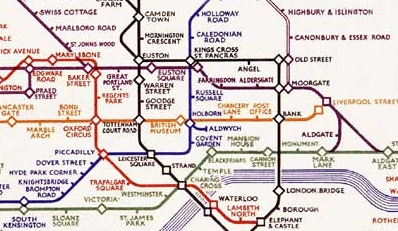
\includegraphics[width=0.9\textwidth]{beck_1933_map}
  \caption[1933 London Underground Tube map]{%
    The present Underground Tube map of London was introduced as early as
    1933 by graphic designer Harry Beck. It's merits are discussed
    with regards to visual design by \citet{hadlaw03} and highlighted as
    a remarkable example of abstraction in relation to computing by
    \citet{kramer07}. Retrieved from the Transport for London web site:
    \url{http://www.tfl.gov.uk/beckmap1.jpg}.}
  \label{figure:beck.1933.map}
\end{figure}

No maps are available yet since the author don't have access to the required
\emph{Adobe Illustrator} software.

    \end{appendices}
  \backmatter
    \bibliographystyle{kluwer}
    \bibliography{bibliography}
\end{document}
